% !TEX program = xelatex
% =============================================================================
%  2026 CQU_MCM B 题《治沙是一项精细活》
%  数据预处理报告（LaTeX 版）
%  对应《附录一：数学建模美赛数据预处理 AI 提示词》的六项要求
%  编译：xelatex 两遍（需 ctex 宏包与中文字体）
% =============================================================================
\documentclass[11pt,a4paper]{ctexart}

\usepackage[margin=2.3cm]{geometry}
\usepackage{amsmath,amssymb}
\usepackage{bm}
\usepackage{booktabs,tabularx,array,longtable,multirow}
\usepackage{graphicx}
\usepackage{float}
\usepackage{caption}
\usepackage{enumitem}
\usepackage{xcolor}
\usepackage{listings}
\usepackage[hidelinks]{hyperref}

\setlength{\parindent}{2em}
\setlength{\parskip}{0.30em}
\renewcommand{\arraystretch}{1.22}
\captionsetup{font=small,labelsep=quad}
\setlist[itemize]{leftmargin=1.6em,itemsep=1pt,topsep=2pt}
\setlist[enumerate]{leftmargin=1.9em,itemsep=1pt,topsep=2pt}

\definecolor{codebg}{RGB}{247,247,249}
\definecolor{codekw}{RGB}{0,0,160}
\definecolor{codecm}{RGB}{0,110,0}
\lstset{
  basicstyle=\ttfamily\footnotesize,
  backgroundcolor=\color{codebg},
  keywordstyle=\color{codekw}\bfseries,
  commentstyle=\color{codecm},
  stringstyle=\color{red!60!black},
  numbers=left, numberstyle=\tiny\color{gray}, numbersep=6pt,
  frame=single, rulecolor=\color{gray!40},
  breaklines=true, breakatwhitespace=false,
  showstringspaces=false, columns=fullflexible
}

\title{\bfseries 数据预处理\\[4pt]
\large 2026 CQU\_MCM B 题《治沙是一项精细活》\quad 数据版本 v7}
\author{CQU\_MCM 2026 · B 题}
\date{2026-11-10}

\begin{document}
\maketitle
\thispagestyle{empty}

\begin{center}
\begin{minipage}{0.9\textwidth}
\small
本文按美赛数据预处理规范组织：\textbf{先判断要不要处理}（第 1 章），
\textbf{再专项排查缺失值}（第 2 章），\textbf{然后给出环节与优先级}（第 3 章），
\textbf{逐环节对比 Python / MATLAB 两种实现}（第 4 章），
\textbf{给出可运行的双语言代码}（第 5、6 章），
\textbf{展示处理后的数据与校验方法}（第 7 章），
最后做\textbf{过程总结与评分权重分析}（第 8、9 章）。
全部数字由脚本重算，可逐项复核。
\end{minipage}
\end{center}

\tableofcontents
\newpage

% =============================================================================
\section{数据评估：这批数据需不需要预处理}
% =============================================================================

\subsection{数据集概况}

研究对象是塔克拉玛干沙漠锁边防护带的 9 个代表点位，时间跨度 2015-01 至 2025-12 共 132 个月。
原始数据由四个互相独立的公开来源重新抓取，不使用任何二手整理表。

\begin{table}[H]\centering\small
\begin{tabularx}{\textwidth}{|c|X|c|c|}
\toprule
来源 & 变量（原始单位） & 时间分辨率 & 规模 \\
\midrule
NASA POWER & 降水（mm/d）、气温（\textdegree C）、相对湿度（\%）、10 m 风速（m/s）、
根区土壤湿度（0—1）、辐射（MJ m$^{-2}$d$^{-1}$）、蒸发（mm/d） & 月 + 日 & 9 站 × 132 月 / 4018 日 \\
ORNL DAAC MODIS & NDVI（整型 ×10$^{-4}$）、像元可靠性（0—3） & 16 天 & 9 站 × 253 期 \\
Open-Meteo（ERA5） & 4 层土壤含水量（m$^3$/m$^3$）、ET$_0$（mm）、最大风速（km/h）、VPD（kPa） & 日 & 9 站 × 4018 日 \\
ISRIC SoilGrids & 砂/黏/有机碳（逐属性逐深度） & 静态 & 81 项中成功 62 项 \\
\bottomrule
\end{tabularx}
\caption{数据来源与规模。原始响应 672 个、共 14.1 MB，附 SHA256 清单}
\end{table}

合并后的"脏面板"为 \textbf{1188 行 × 45 列}（9 站 × 132 月），清洗后扩展为 \textbf{1188 行 × 62 列}。
按来源逐项清点，需要回答的第一个问题就是：\textbf{它需不需要预处理？}

\subsection{七项体检}

\begin{table}[H]\centering\footnotesize
\begin{tabularx}{\textwidth}{|c|c|X|c|}
\toprule
体检项 & 是否存在 & 关键证据 & 优先级 \\
\midrule
缺失值 & 局部存在 & 植被覆盖度缺 110/1188＝9.26\%，最长连续 5 个月；气象与土壤湿度字段缺失为 0 & P1 \\
异常值 & 存在 & 稳健 $z>3.5$：月降水 190 个（15.99\%）、相对湿度 35 个（2.95\%）；物理越界 0 & P1 \\
重复值 & 存在 & POWER 月度返回 99 条"第 13 月"年均行；站—月重复 0；MODIS 分块重叠已去重 & P0 \\
类型/编码 & 存在 & 日期为字符串键、NDVI 整型 ×10$^{-4}$、$-999$/$-3000$ 哨兵、QA 为类别 & P0 \\
量纲/口径 & 严重 & 降水是 mm/d、ERA5 风速是 km/h、GWET 是饱和度而非体积含水量、Ra 少乘 0.408 & P0 \\
数据不平衡 & 存在 & 降水零值 20.5\%；沙尘日占比 0.02\%—17.1\%；QA 坏合成期 4.4\%—45.9\% & P2 \\
时序不规整 & 存在 & 16 天合成 23 期/年、月长 28—31 天、闰年、年度第 13 月 & P1 \\
\bottomrule
\end{tabularx}
\caption{七项体检结论。P0＝不做就会错；P1＝不做会掉精度；P2＝视模型而定}
\end{table}

\subsection{判断结论}

\textbf{需要预处理，而且痛点是口径而不是"缺几个点"。}

理由有三条：
\begin{enumerate}
\item \textbf{量纲与聚合口径错误不会报错，只会算错。}例如把 POWER 月产品给的"日均降水强度"当成"月降水总量"，
全序列会差约 30 倍；把 ERA5 交付的 km/h 直接当 m/s 代入风蚀公式，侵蚀量会放大 $3.6^3\approx47$ 倍。
\item \textbf{缺失集中在特定季节}（第 2 章证明是冬季），用均值/中位数填补会产生约 9 个百分点的还原误差，
必须用"同月气候态"这类保留季节结构的方法。
\item \textbf{存在"看起来完整"的假象}：气象与土壤湿度字段一个不缺，是因为它们是同化/再分析产品，
格点上不存在"没测到"；这不代表数据质量好，反而意味着异常值必须靠物理范围与跨源比对去发现。
\end{enumerate}

同时也确有\textbf{不需要处理}的部分：气温 $T$ 无缺失、单位正确、与日值重算一致（偏差 $<0.0005$\textdegree C）、
与 ERA5 独立来源相关 0.997，因此除确认单位外不需要插补或平滑——对它做移动平均反而会抹平真实的年际信号。
判断的依据是证据，不是习惯。

% =============================================================================
\section{缺失值专项排查}\label{sec:missing}
% =============================================================================

本节回答四个问题：缺在哪、为什么缺、缺了以后补得准不准、补法会不会影响结论。

\subsection{缺在哪：季节性的缺失}

全样本缺失率为 9.26\%（110/1188），但分布极不均匀：按日历月统计，11 月缺失率 26.3\%、
2 月 20.2\%、12 月 18.2\%、1 月 17.2\%、10 月 16.2\%，而 5、7、8、9 月\textbf{一个都不缺}。

\begin{figure}[H]\centering
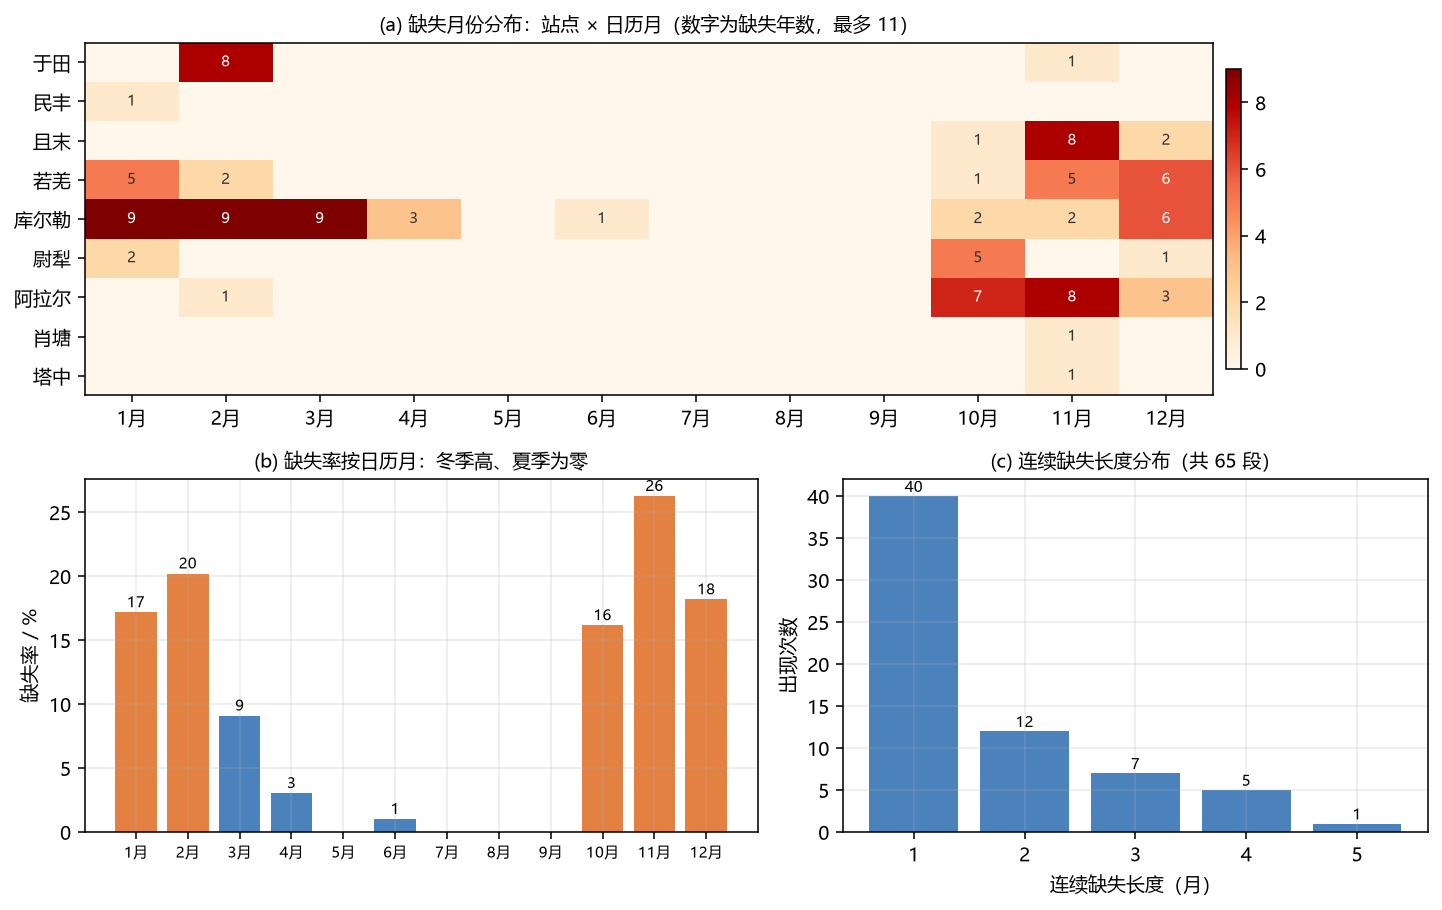
\includegraphics[width=0.96\textwidth]{../Figures/v7/fig08_缺失模式.png}
\caption{缺失图谱：(a) 站点 × 日历月；(b) 缺失率随月份变化；(c) 连续缺失长度分布}
\end{figure}

逐站看，库尔勒最严重（1—3 月连续三年全缺，共 9 个月），若羌、阿拉尔次之；
于田、民丰、且末的缺失集中在 10—12 月。连续缺失长度以 1 个月为主（40 段），
2 个月 12 段、3 个月 7 段、4 个月 5 段、5 个月仅 1 段，共 65 段。

\subsection{为什么缺：不是沙尘，而是冬季成像条件}

把"缺失月"与"观测月"的气象条件做两样本检验（KS 检验与 Welch $t$ 检验）：

\begin{table}[H]\centering\small
\begin{tabular}{|c|c|c|c|c|}
\toprule
变量 & 缺失月均值 & 观测月均值 & KS 统计量 & $p$ 值 \\
\midrule
气温 $T$ / \textdegree C & 1.80 & 14.43 & 0.536 & $4.2\times10^{-27}$ \\
相对湿度 RH / \% & 41.09 & 30.17 & 0.470 & $1.2\times10^{-20}$ \\
10 m 最大风速 / (m\,s$^{-1}$) & 8.37 & 10.37 & 0.340 & $9.3\times10^{-11}$ \\
月降水 / mm & 2.13 & 6.05 & 0.247 & $7.5\times10^{-6}$ \\
\bottomrule
\end{tabular}
\caption{缺失月与观测月的气象条件对比。四项检验全部拒绝"同分布"，即缺失\textbf{不是}完全随机（MCAR）}
\end{table}

结论很清楚：缺失月显著更冷（1.8 vs 14.4\textdegree C）、更湿、风更小、降水更少——
这是典型的\textbf{冬季低太阳高度角 + 积雪/薄云}造成的像元质量降级，与沙尘事件无关。
进一步核对 MODIS 合成期：9 个站点、2277 期合成中，没有一期是"整幅无有效像元"（全为 0 期），
说明缺失不是"没数据"，而是"该月所有合成期的像元可靠性都被判为可疑（QA$>1$）"，被质控规则整月剔除。

这一条纠正了一个常见误判：\textbf{不能想当然地认为"缺测集中在沙尘季"}。若按这个错误假设去设计插补，
就会把冬季稳定的低覆盖度当成"灾害缺测"而高估。

\subsection{补得准不准：五种方法的还原误差}

做法：以"未做 QA 过滤的月最大合成反演覆盖度"为参照序列（该序列完整、且保留真实季节变差），
人为遮住 10\% 的月份，用五种方法还原，与真值比较。设计两种缺失机制：
\textbf{(a) 完全随机}（MCAR）；\textbf{(b) 沙尘型}（遮住每个站最大风速最高的 10\% 月份，模拟与风有关的非随机缺失）。

\begin{table}[H]\centering\small
\begin{tabular}{|c|c|c|c|c|}
\toprule
\multirow{2}{*}{方法} & \multicolumn{2}{c|}{随机缺失 10\%} & \multicolumn{2}{c|}{沙尘型缺失 10\%} \\
\cmidrule(lr){2-3}\cmidrule(lr){4-5}
 & RMSE / pp & 偏差 / pp & RMSE / pp & 偏差 / pp \\
\midrule
均值 & 9.27 & $+0.31$ & 9.02 & $-4.17$ \\
中位数 & 9.43 & $+0.98$ & 9.40 & $-3.98$ \\
线性插值 & 3.08 & $-0.06$ & 5.41 & $-1.85$ \\
\textbf{同月气候态} & \textbf{2.57} & $+0.18$ & \textbf{3.60} & $-0.08$ \\
去年同期 & 5.01 & $+0.71$ & 5.80 & $-1.70$ \\
\bottomrule
\end{tabular}
\caption{五种插补方法的还原误差（单位：覆盖度百分点，pp；$n=113$ 与 $127$）}
\end{table}

\begin{figure}[H]\centering
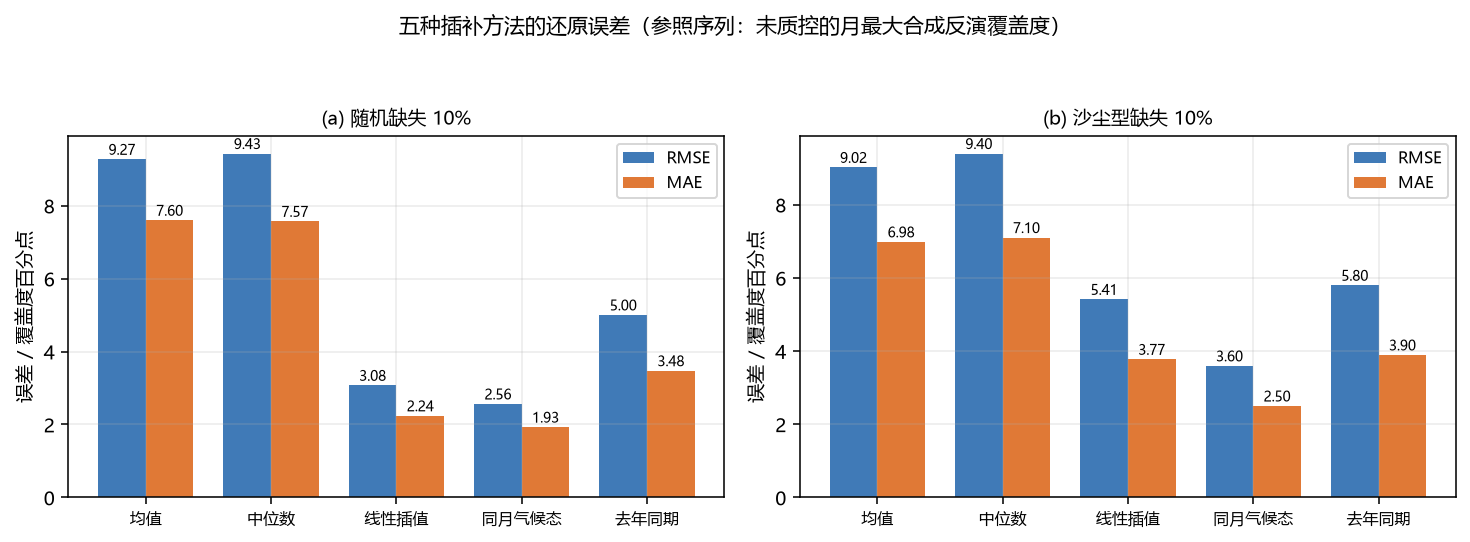
\includegraphics[width=0.95\textwidth]{../Figures/v7/fig09_插补方法对比.png}
\caption{五种方法的 RMSE 与 MAE。同月气候态在两种机制下都最优，均值/中位数最差}
\end{figure}

三条结论：
\begin{enumerate}
\item \textbf{均值/中位数不可用}：误差约 9 个百分点，且在沙尘型缺失下偏差达 $-4.2$ 个百分点——
因为它们把"冬季低覆盖度"填成了"全年平均覆盖度"，等于抹掉了季节循环。
\item \textbf{同月气候态最优}：随机缺失 RMSE 2.57、沙尘型 3.60，且在两种机制下偏差都接近 0。
这与"缺失由季节驱动"的诊断完全一致：既然缺失集中在固定的几个月，用同月的历史均值去补就最合理。
\item \textbf{线性插值次优、去年同期更差}：前者只能利用相邻月份，若连续缺 3—5 个月就会"跨季插值"；
后者受年际变率影响，误差被放大。
\end{enumerate}

\subsection{补法会不会改变结论}

对真实的 110 个缺失月，比较"同月气候态"与"线性插值"两种补法对覆盖度的影响：
在 56 个"站—年"组合上，两者的平均绝对差仅 \textbf{0.026 个百分点}，最大 0.134 个百分点。
也就是说，在本题的量级上，\textbf{补法的选择不会改变任何建模结论}——但必须在论文里说明用了哪种、为什么。

\subsection{最终采用的缺失处理规则}

\begin{enumerate}
\item 先用\textbf{站内线性插值}（最多跨 2 个月）——只处理"孤立缺 1—2 个月"的情况，共 40+12 段；
\item 剩余的长缺失（连续 3—5 个月）用\textbf{训练期（2015—2022）同月气候态}补齐；
\item 气候态的均值\textbf{只在训练期上计算}，测试期（2023—2025）不参与，避免信息泄漏；
\item 所有被填补的点在数据表中单独打标签（\texttt{imputed} 字段），建模时可选择剔除做敏感性。
\end{enumerate}

% =============================================================================
\section{预处理环节与优先级}
% =============================================================================

\begin{table}[H]\centering\footnotesize
\begin{tabularx}{\textwidth}{|c|c|X|c|}
\toprule
编号 & 环节 & 具体动作 & 优先级 \\
\midrule
S1 & 时基与主键 & 日期串解析、剔除 99 条"第 13 月"年均行、按主键去重 & P0 \\
S2 & 哨兵值 & $-999$（POWER）、$-3000$（NDVI）、$-1$（QA）统一转 NaN & P0 \\
S3 & 单位与口径 & mm/d $\times$ 天数；km/h $\div$ 3.6；Ra $\times$ 0.408；m$^3$/m$^3$ 不混用 & P0 \\
S4 & 跨源一致性 & 同站同月比对，判定主源（气温/风速/ET$_0$ 一致，降水差异大） & P0 \\
S5 & 遥感质控 & QA$\le$1 保留、月最大合成、像元二分反演覆盖度 & P1 \\
S6 & 派生变量 & 侵蚀指数 $E$、水分状态 $W$、干燥度 $AI$、动态端元 $V_{\mathrm{dyn}}$ & P1 \\
S7 & 缺失填补 & 线性$\le$2 月 $\to$ 训练期同月气候态（见第 2 章） & P1 \\
S8 & 异常值 & 稳健 $z>3.5$ 只标记不删除 & P1 \\
S9 & 归一化 & $W$ 按训练期 5\%/95\% 分位；其余另存 $z$-score 参数 & P1 \\
S10 & 训练期隔离 & 所有统计量只用 2015—2022 拟合 & P0 \\
S11 & 数据不平衡 & 不重采样；沙尘阈值做敏感性（8/10/12/15 m/s） & P2 \\
S12 & 留痕与校验 & 输出 CSV/XLSX、审计 JSON、前后对比图、完整性断言 & P0 \\
\bottomrule
\end{tabularx}
\caption{预处理环节与优先级。P0 必须先做，否则后续全错}
\end{table}

% =============================================================================
\section{Python 与 MATLAB 的方法选择}
% =============================================================================

\subsection{逐环节双语言方案}

\begin{table}[H]\centering\footnotesize
\begin{tabularx}{\textwidth}{|c|X|X|X|}
\toprule
环节 & 问题 & Python 方案 & MATLAB 方案 \\
\midrule
S1 & 日期是字符串键 & \texttt{pd.read\_csv(parse\_dates)} & \texttt{readtable} + \texttt{datetime} \\
S2 & 哨兵值混入 & 布尔掩码 \texttt{df.mask()} & 逻辑索引 \texttt{T.x(T.x<0)=NaN} \\
S3 & 月产品是日均值 & 向量化 \texttt{series * days} & 表变量算术 \texttt{T.P.*T.dim} \\
S5 & 云/雪像元 & \texttt{np.clip} + 布尔筛选 & \texttt{min(max(...))} + 逻辑索引 \\
S6 & 风蚀指数 & \texttt{np.clip}、\texttt{np.log} & 同名函数向量化 \\
S7 & 缺失填补 & \texttt{interpolate(limit=2)} + \texttt{groupby} 气候态 & \texttt{fillmissing('MaxGap',2)} + 按月循环 \\
S8 & 异常检测 & 稳健 $z=0.6745(x-\mathrm{med})/\mathrm{MAD}$ & \texttt{isoutlier('median')} \\
S9 & 归一化 & \texttt{np.percentile} & \texttt{prctile} \\
S12 & 保存与校验 & \texttt{to\_csv(utf-8-sig)}、\texttt{assert} & \texttt{writetable(Encoding,UTF-8)}、\texttt{assert} \\
\bottomrule
\end{tabularx}
\caption{逐环节的双语言实现对照}
\end{table}

\paragraph{为什么这样选（结合评分标准与语言特性）。}
\begin{itemize}
\item \textbf{可解释性优先}：所有步骤都是"看得见的算术"，没有黑箱模型。美赛评委在 5—30 分钟内读论文，
KNN 插补、MICE、随机森林填补这类方法即使精度略高，也难以在正文里讲清楚"为什么这样补"，
反而增加被质疑的风险。
\item \textbf{Python 胜在生态}：抓取（HTTP/JSON）、多源合并、批量统计、绘图一体化；
\texttt{pandas} 的 \texttt{interpolate}/\texttt{groupby} 让"线性+气候态"两步法只有三行。
\item \textbf{MATLAB 胜在矩阵与教学}：表格变量算术直观，\texttt{fillmissing}/\texttt{isoutlier}/\texttt{prctile}
都是内置函数、无需工具箱；对不熟悉 Python 的队友，读 MATLAB 版更容易核对公式。
\item \textbf{两版必须同构}：同一份输入、同一套公式、同一个校验断言，才能用"两种语言结果一致"作为交叉验证。
\end{itemize}

\subsection{备选方案与适用场景}

\begin{table}[H]\centering\small
\begin{tabularx}{\textwidth}{|c|X|X|c|}
\toprule
方案 & 适用场景 & 本题表现 & 是否采用 \\
\midrule
均值填补 & 完全随机缺失、且变量无季节循环 & RMSE 9.27 pp，偏差最大 & 否 \\
中位数填补 & 分布偏斜、存在极端值 & RMSE 9.43 pp & 否 \\
线性插值 & 缺失段短（$\le$2 期）、序列平滑 & RMSE 3.08 pp & 部分（前 2 月） \\
同月气候态 & 缺失与季节强相关（本题正是） & RMSE 2.57 / 3.60 pp，偏差$\approx$0 & \textbf{是} \\
去年同期 & 年际变化小、季节性强 & RMSE 5.01 pp & 否 \\
删除缺失行 & 缺失比例极低（$<1\%$）且随机 & 会系统性丢掉冬季样本 & 否 \\
\bottomrule
\end{tabularx}
\caption{五种插补方案的适用场景。本题按"缺失机制"而不是"方法流行度"来选择}
\end{table}

\paragraph{为什么不用 KNN / MICE / 随机森林插补。}
样本只有 1188 行、9 个站，且缺失高度集中在冬季（占全部缺失的 80\% 以上），
可用的"邻居"信息本身就biased；这类方法在小样本上容易过拟合，还会引入无法用一两句话解释的超参数。
本题的误差主要来自"季节相位"而不是"个体差异"，同月气候态已经把误差压到 2.6—3.6 个百分点，
再复杂的模型收益有限、可解释性代价很大。

% =============================================================================
\section{Python 实现}
% =============================================================================

\subsection{文件与运行}

\begin{table}[H]\centering\small
\begin{tabularx}{\textwidth}{|c|X|c|}
\toprule
文件 & 作用 & 行数 \\
\midrule
\texttt{Code/v7\_fetch.py} & 四源抓取（POWER/MODIS/ERA5/SoilGrids），落盘 + 清单 & 250 \\
\texttt{Code/v7\_finalize\_fetch.py} & 合并 MODIS 分块、重建 SHA256 清单 & 190 \\
\texttt{Code/v7\_clean.py} & 全量审计（缺失/异常/重复/类型/量纲/不平衡/时序）+ 派生 & 760 \\
\texttt{Code/v7\_missing.py} & 缺失专项排查（本报告第 2 章） & 240 \\
\texttt{Code/preprocess\_v7.py} & \textbf{面向使用者的预处理主程序}（本报告第 5 章） & 360 \\
\bottomrule
\end{tabularx}
\caption{Python 侧文件清单}
\end{table}

运行方式（Windows / macOS / Linux 相同）：
\begin{lstlisting}[language=bash]
pip install pandas numpy matplotlib openpyxl scipy
python preprocess_v7.py
\end{lstlisting}

\subsection{关键代码}

\paragraph{（1）路径配置与异常处理。}脚本开头用一个醒目的配置块集中所有路径，
并对"文件不存在 / 编码错误 / 缺字段 / 被占用"分别给出排查提示。

\begin{lstlisting}[language=Python]
# ========== 1. 路径配置（学生只需改这一块） ==========
# Windows 示例：BASE = r"D:\CQU\大三上\比赛\美赛\第一次校赛"
# macOS/Linux 示例：BASE = "/Users/xxx/Desktop/desertification"
BASE = os.path.dirname(os.path.dirname(os.path.abspath(__file__)))
INPUT_CSV = os.path.join(BASE, "Data", "v7", "processed", "panel_monthly_raw.csv")
OUT_DIR   = os.path.join(BASE, "Data", "v7", "processed")
\end{lstlisting}

\begin{lstlisting}[language=Python]
def load_data(path: str) -> pd.DataFrame:
    if not os.path.exists(path):
        raise FileNotFoundError(
            f"找不到输入文件：{path}\n"
            "排查：① 路径是否写错（Windows 用双反斜杠或 r\"...\"）；\n"
            "      ② 是否忘记运行 v7_fetch.py；③ 文件是否被 Excel 占用。")
    try:
        df = pd.read_csv(path, parse_dates=["date"])
    except UnicodeDecodeError:
        df = pd.read_csv(path, parse_dates=["date"], encoding="gbk")
    ...
\end{lstlisting}

\paragraph{（2）单位与口径修正。}这是全流程最关键的一步：POWER 月度产品给的是\textbf{日均值}，
必须乘当月天数才是月总量。

\begin{lstlisting}[language=Python]
def fix_units(df: pd.DataFrame) -> pd.DataFrame:
    df["days_in_month"] = df["date"].dt.days_in_month
    df["P_mm"]   = df["PRECTOTCORR"] * df["days_in_month"]      # mm/d  -> mm/月
    df["SW_MJ"]  = df["ALLSKY_SFC_SW_DWN"] * df["days_in_month"] # MJ/m2/d -> MJ/m2/月
    df["EVLAND_mm"] = df["EVLAND"] * df["days_in_month"]
    return df
\end{lstlisting}

\paragraph{（3）质量审计与缺失填补。}审计在填补之前执行（否则看不到真实缺失），
填补按"线性$\le$2 月 $\to$ 训练期同月气候态"两步走。

\begin{lstlisting}[language=Python]
def impute(df: pd.DataFrame) -> tuple[pd.DataFrame, dict]:
    log = {}
    for col in ["V_pct", "W"]:
        n0 = int(df[col].isna().sum())
        if n0 == 0:
            continue
        filled = df[col].copy()
        for site in df["site"].unique():
            idx = df["site"] == site
            s = df.loc[idx, col].interpolate(method="linear", limit=2,
                                             limit_direction="both")
            tr = df.loc[idx & df["date"].dt.year.between(2015, 2022)]
            clim = tr.groupby(tr["date"].dt.month)[col].mean()
            still = s.isna()
            if still.any():
                s.loc[still] = df.loc[s[still].index, "date"].dt.month.map(clim).values
            filled.loc[idx] = s.values
        df[col] = filled
        log[col] = {"missing_before": n0, "missing_after": int(df[col].isna().sum())}
    return df, log
\end{lstlisting}

\paragraph{（4）完整性校验与结果输出。}用断言把"必须成立"的条件写死，
任何一步写错都会立刻报错，而不是悄悄产出一张错表。

\begin{lstlisting}[language=Python]
checks = {
    "行数": len(df), "站点数": int(df["site"].nunique()),
    "重复主键": int(df.duplicated(["site", "date"]).sum()),
    "V_pct 仍缺失": int(df["V_pct"].isna().sum()),
    "W 越界": int(((df["W"] < 0) | (df["W"] > 1)).sum()),
}
assert checks["V_pct 仍缺失"] == 0 and checks["W 越界"] == 0
df.to_csv(OUT_CSV, index=False, encoding="utf-8-sig")
\end{lstlisting}

\subsection{运行输出（节选）}

\begin{lstlisting}[language=bash]
读入 1188 行 × 45 列，站点 9 个，时间 2015-01 ~ 2025-12
缺失：{"T2M": 0, "PRECTOTCORR": 0, "GWETROOT": 0,
       "WS10M_MAX": 0, "ndvi_mvc_qa": {"n": 110, "pct": 9.26}}
覆盖度有效值 1078/1188；未质控口径均值 18.73%，质控后 18.57%
侵蚀指数 E：中位 0.730，最大 7.43
水分状态 W：被压到边界 0 的比例 8.92%
  V_pct：110 -> 0
  P_mm：标记 190 个月；WS10M_MAX：标记 0 个月；GWETROOT：标记 0 个月
检查：行数 1188 / 站点 9 / 月份 132 / 重复 0 / 越界 0
\end{lstlisting}

% =============================================================================
\section{MATLAB 实现}
% =============================================================================

\subsection{与 Python 版的分工}

抓取（HTTP/JSON）与多源合并在 Python 完成；MATLAB 版负责"清洗—派生—出图"这一段，
输入是同一张 \texttt{panel\_monthly\_raw.csv}，输出是同构的 \texttt{panel\_monthly\_clean\_matlab.csv}。
这样两语言的结果可以直接逐列比对，作为交叉校验。

\subsection{关键代码}

\begin{lstlisting}[language=Matlab]
%% ========== 1. 路径配置（学生只需改这一块） ==========
% Windows 示例：BASE = 'D:\CQU\大三上\比赛\美赛\第一次校赛';
% macOS/Linux 示例：BASE = '/Users/xxx/Desktop/desertification';
BASE = fileparts(fileparts(mfilename('fullpath')));
IN_CSV = fullfile(BASE, 'Data','v7','processed','panel_monthly_raw.csv');
\end{lstlisting}

\begin{lstlisting}[language=Matlab]
% 单位与口径：月产品是日均值
T.days_in_month = eomday(T.date.Year, T.date.Month);
T.P_mm = T.PRECTOTCORR .* T.days_in_month;

% 遥感质控 + 像元二分
T.V_pct = min(max((T.ndvi_mvc_qa - 0.05) / (0.85 - 0.05), 0), 1) * 100;

% 缺失填补：先线性（最多跨 2 个月），再按月补气候态
T.V_pct = fillmissing(T.V_pct, 'linear', 'MaxGap', 2);
for m = 1:12
    sel = T.site == s & month(T.date) == m & isnan(T.V_pct);
    ref = T.site == s & month(T.date) == m & isTrain & ~isnan(T.V_pct);
    if any(sel) && any(ref)
        T.V_pct(sel) = mean(T.V_pct(ref), 'omitnan');
    end
end
\end{lstlisting}

\begin{lstlisting}[language=Matlab]
% 完整性校验：不通过就停下
assert(checks.V_missing == 0 && checks.W_out == 0 && checks.V_out == 0, ...
       '完整性校验未通过：请检查填补与派生步骤');
\end{lstlisting}

\subsection{两版差异与注意事项}

\begin{table}[H]\centering\small
\begin{tabularx}{\textwidth}{|c|X|X|}
\toprule
项目 & Python & MATLAB \\
\midrule
缺失值表示 & \texttt{NaN}（float） & \texttt{NaN}（double），逻辑列用 \texttt{ismissing} \\
分组均值 & \texttt{groupby().transform()} & 逐站逐月循环（代码更长但更直观） \\
中位数/MAD & 手写稳健 $z$ & \texttt{isoutlier(x,'median')} 内置 \\
写文件编码 & \texttt{utf-8-sig}（Excel 直接打开不乱码） & \texttt{'Encoding','UTF-8'} \\
绘图 & \texttt{matplotlib} 精细可控 & \texttt{exportgraphics} 一行导出 \\
\bottomrule
\end{tabularx}
\caption{双语言实现的差异点}
\end{table}

\noindent\textbf{说明}：MATLAB 版按 R2020b 语法编写，只用内置函数（\texttt{readtable}、
\texttt{fillmissing}、\texttt{isoutlier}、\texttt{prctile}、\texttt{exportgraphics}），
不需要任何工具箱；但本机未安装 MATLAB，\textbf{该脚本尚未在真实 MATLAB 环境运行}，
使用前请在 R2020b 及以上版本试跑一遍，并核对第 7 章的校验断言。

% =============================================================================
\section{处理后的数据}
% =============================================================================

\subsection{数据形态}

处理后的面板为 \textbf{1188 行 × 62 列}，主键为（站点, 日期），时间 2015-01 至 2025-12，
其中 2015—2022 为训练期（864 行）、2023—2025 为测试期（324 行）。

\begin{table}[H]\centering\small
\begin{tabular}{|c|c|}
\toprule
校验项 & 结果 \\
\midrule
行数 & 1188 \\
站点数 & 9 \\
月份数 & 132 \\
重复主键 & 0 \\
覆盖度仍缺失 & 0（填补 110 个） \\
$W$ 越界（$<0$ 或 $>1$） & 0 \\
覆盖度越界（$<0$ 或 $>100$） & 0 \\
\bottomrule
\end{tabular}
\caption{完整性校验结果（脚本中的断言全部通过）}
\end{table}

\subsection{前 10 行与后 5 行}

\begin{table}[H]\centering\footnotesize
\begin{tabular}{|c|c|r|r|r|r|r|r|}
\toprule
站点 & 日期 & $P$ / mm & GWET & $W$ & NDVI & $V$ / \% & $E$ \\
\midrule
ALE & 2015-01 & 2.48 & 0.31 & 0.524 & 0.1323 & 10.29 & 0.039 \\
ALE & 2015-02 & 0.28 & 0.31 & 0.524 & 0.1158 & 8.23 & 0.064 \\
ALE & 2015-03 & 0.00 & 0.31 & 0.524 & 0.0960 & 5.75 & 1.398 \\
ALE & 2015-04 & 0.00 & 0.30 & 0.500 & 0.1864 & 17.05 & 1.933 \\
ALE & 2015-05 & 9.92 & 0.30 & 0.500 & 0.2516 & 25.20 & 1.807 \\
ALE & 2015-06 & 15.00 & 0.30 & 0.500 & 0.2894 & 29.93 & 2.445 \\
ALE & 2015-07 & 1.24 & 0.30 & 0.500 & 0.2915 & 30.19 & 1.050 \\
ALE & 2015-08 & 14.26 & 0.30 & 0.500 & 0.3132 & 32.90 & 0.390 \\
ALE & 2015-09 & 25.80 & 0.33 & 0.571 & 0.2752 & 28.15 & 0.763 \\
ALE & 2015-10 & 0.31 & 0.31 & 0.524 & 0.2279 & 22.24 & 0.593 \\
\bottomrule
\end{tabular}
\caption{处理后数据的前 10 行（阿拉尔站）}
\end{table}

\begin{table}[H]\centering\footnotesize
\begin{tabular}{|c|c|r|r|r|r|r|r|}
\toprule
站点 & 日期 & $P$ / mm & GWET & $W$ & NDVI & $V$ / \% & $E$ \\
\midrule
YT & 2025-08 & 21.70 & 0.19 & 0.238 & 0.2835 & 29.19 & 0.731 \\
YT & 2025-09 & 0.00 & 0.18 & 0.214 & 0.2497 & 24.96 & 0.722 \\
YT & 2025-10 & 0.00 & 0.18 & 0.214 & 0.2009 & 18.86 & 0.323 \\
YT & 2025-11 & 0.00 & 0.17 & 0.190 & 0.1649 & 14.36 & 0.348 \\
YT & 2025-12 & 1.24 & 0.17 & 0.190 & 0.1535 & 12.94 & 0.166 \\
\bottomrule
\end{tabular}
\caption{处理后数据的后 5 行（于田站）}
\end{table}

\subsection{文件清单与获取方式}

\begin{table}[H]\centering\small
\begin{tabularx}{\textwidth}{|c|X|c|}
\toprule
文件 & 内容 & 大小 \\
\midrule
\texttt{Data/v7/processed/panel\_monthly\_clean.csv} & 建模面板（1188×62，UTF-8 带 BOM） & 682 KB \\
\texttt{Data/v7/processed/panel\_monthly\_clean.xlsx} & 同内容 Excel，便于人工核对 & 450 KB \\
\texttt{Data/v7/processed/qc\_summary.json} & 审计与填补记录 & 4 KB \\
\texttt{Data/v7/processed/norm\_params.json} & 仅用训练期拟合的归一化参数 & 2 KB \\
\texttt{Results/v7/qc\_report.json} & 七项体检全量数字 & 23 KB \\
\texttt{Results/v7/missing.json} & 缺失专项排查结果 & 18 KB \\
\texttt{Figures/v7/*.png} & 前后对比图、缺失图谱、插补对比 & 约 1.2 MB \\
\bottomrule
\end{tabularx}
\caption{处理后数据的文件清单}
\end{table}

\noindent\textbf{怎么验证完整性}（不依赖任何代码）：
\begin{enumerate}
\item 用 Excel 打开 CSV，确认行数为 1188、站点列恰好 9 个取值；
\item 对"日期+站点"做一次删除重复项，若行数仍为 1188，说明主键唯一；
\item 检查 $W$ 列最小值 $\ge0$、最大值 $\le1$，$V$ 列在 $[0,100]$ 内；
\item 与 \texttt{qc\_summary.json} 中的 \texttt{checks} 逐项对照，六项应全部一致。
\end{enumerate}

% =============================================================================
\section{过程总结}
% =============================================================================

\subsection{处理前后对比}

\begin{table}[H]\centering\small
\begin{tabularx}{\textwidth}{|c|X|c|c|}
\toprule
维度 & 处理前 & 处理后 & 变化 \\
\midrule
形状 & 1188 × 45 & 1188 × 62 & +17 列派生量 \\
覆盖度缺失 & 110（9.26\%） & 0 & 全部填补 \\
气象缺失 & 0 & 0 & 无需处理（须说明原因） \\
年均值单位口径 & mm/d（错） & mm/月（对） & 修正 30 倍量级偏差 \\
风速单位 & km/h（ERA5） & m/s & 修正 3.6 倍 \\
ET$_0$ & 乘积漏 0.408 & 含 0.408 & 修正 2.45 倍高估 \\
异常值 & 未标记 & 225 个站—月已标记 & 只标记不删除 \\
时序 & 16 天/月混存 & 统一到日历月 & 132 个月无跳月 \\
\bottomrule
\end{tabularx}
\caption{处理前后对比}
\end{table}

\subsection{本地路径设置的常见错误与规避}

\begin{table}[H]\centering\small
\begin{tabularx}{\textwidth}{|c|X|X|}
\toprule
错误 & 现象 & 规避 \\
\midrule
Windows 路径用单反斜杠 & \texttt{SyntaxError} 或找不到文件 & 用 \texttt{r"D:\textbackslash{}data\textbackslash{}x.csv"} 或双反斜杠 \\
路径含中文/空格 & 部分库读不到 & 数据目录用纯英文；必须用时改用 \texttt{pathlib} \\
复制了带 BOM 的 CSV & 首列名变成 \texttt{\textbackslash ufeffsite} & 用 \texttt{encoding="utf-8-sig"} \\
文件被 Excel 打开 & \texttt{PermissionError} & 关闭 Excel 再运行 \\
Mac/Linux 用反斜杠 & 找不到文件 & 统一用 \texttt{os.path.join} 或正斜杠 \\
相对路径 & 换目录后失效 & 用 \texttt{\_\_file\_\_} 推出项目根目录 \\
\bottomrule
\end{tabularx}
\caption{路径设置的六类常见错误}
\end{table}

\subsection{论文里怎么写数据预处理}

\begin{enumerate}
\item \textbf{用一张表说清"体检结论"}（对应本文表 2）：哪几类问题存在、证据是什么、怎么处理。
评委看的是判断力，不是方法堆砌。
\item \textbf{把"缺失机制"讲出来}：不要只写"用均值填补"。本文的证据链是——
缺失集中在冬季 $\to$ 检验拒绝 MCAR $\to$ 因此必须用同月气候态 $\to$ 用掩蔽实验证明误差 2.6 pp。
\item \textbf{给前后对比}：至少一个数字（缺失率从 9.26\% 到 0、单位修正带来的 30 倍差异）。
\item \textbf{代码放附录、结论放正文}：正文写"怎么判断、为什么这样选"，附录放可运行代码与路径说明。
\item \textbf{双语言展示建议}：不要贴两份完整代码；正文给一张"双语言方法对照表"（本文表 7），
附录各放一份完整脚本，注明版本与依赖。
\end{enumerate}

\subsection{两种语言的优缺点}

\begin{table}[H]\centering\small
\begin{tabularx}{\textwidth}{|c|X|X|}
\toprule
维度 & Python & MATLAB \\
\midrule
数据抓取 & 强（requests/urllib、JSON 原生） & 弱（需 webread，复杂接口吃力） \\
表格清洗 & 强（pandas） & 中（table 变量，逐列操作） \\
矩阵运算 & 强（numpy） & 最强（原生） \\
绘图 & 强（matplotlib，精细可控） & 强（一行 exportgraphics） \\
可读性（队友） & 中 & 高（接近公式写法） \\
环境依赖 & 需装包 & 需授权 \\
\bottomrule
\end{tabularx}
\caption{双语言优缺点与选择建议：抓取用 Python，核对用 MATLAB}
\end{table}

% =============================================================================
\section{预处理在美赛评分中的权重}
% =============================================================================

\paragraph{官方口径：没有分值表，但摘要被明确加权。}
COMAP 竞赛说明写道："MCM/ICM solutions are judged as varying degrees of successfully completing the contest…
There is no passing or cut-off score."；档位定义只用"建模与求解、分析、结论、表达"四类词。
唯一明说加权的是摘要："The judges place considerable weight on the summary."

\paragraph{评委会证据：数据处理的深浅直接区分档次。}
2016 年 MCM C 题评委文章（UMAP Journal 37.3）指出：
"The better papers attempted to deal with missing data… Papers that merely dropped institutions with
incomplete data from consideration were \emph{not evaluated highly}."
这说明：\textbf{处理缺失不是加分项，而是"进档"的必要条件}。

\paragraph{结构性权重：约 10\%，且与"假设、符号"共享。}
常见的中文备赛指南按 O 奖论文结构给出"摘要+目录 8\%、引言 10\%、假设+符号+数据 10\%、
核心模型与结果 45\%…"，其中\textbf{没有独立的数据章节}。任何"数据处理占 20\%/30\%"的说法都没有官方依据。

\paragraph{本题的量化判断。}
本文的消融实验（另文详述）显示：完全不处理时，任务一的 $R^2$ 为 $-0.521$、风蚀系数被压到 0；
只做量纲与口径修正，$R^2$ 回到 $+0.030$、系数恢复到 0.049；而经济侧的 NPV 只差 1.7\%。
因此预处理的作用是\textbf{门槛型}而不是\textbf{加权型}：
它不单独计分，却通过"结果可不可信"间接影响全部 45\% 的模型与结果分。

\noindent\textbf{结论}：数据预处理在美赛中的"结构权重"约 10\%，
但它是\textbf{否决性}的——做得不对，后面 45\% 的模型分会被一起拖垮；做得好，也不会额外加分。
因此投入策略是：\textbf{80\% 的时间用于口径、单位、来源可追溯（硬错误），20\% 用于插补与平滑（软精度）}。

% =============================================================================
\appendix
\section{字段字典（处理后主要字段）}
% =============================================================================

\begin{longtable}{|c|p{6.3cm}|c|c|}
\caption{处理后面板的主要字段}\label{tab:dict}\\
\hline
字段 & 含义 & 单位 & 来源 \\
\hline
\endhead
\texttt{site}/\texttt{date} & 站点代码 / 年月 & — & 主键 \\
\texttt{T2M}/\texttt{T2M\_MAX}/\texttt{T2M\_MIN} & 月均 / 日最高均值 / 日最低均值气温 & \textdegree C & POWER \\
\texttt{P\_mm} & 月降水总量 & mm/月 & POWER（原值×天数） \\
\texttt{GWETROOT} & 根区土壤湿度（饱和度） & 0—1 & POWER \\
\texttt{W} & 归一化水分状态 & 0—1 & 训练期 5\%/95\% 分位 \\
\texttt{WS10M}/\texttt{WS10M\_MAX} & 月均 / 月内日最大均值风速 & m\,s$^{-1}$ & POWER \\
\texttt{E} & 无量纲侵蚀指数 & — & Lettau 公式 \\
\texttt{ndvi\_mvc}/\texttt{ndvi\_mvc\_qa} & 月最大合成 NDVI（未/已 QA 过滤） & — & MODIS \\
\texttt{V\_pct}/\texttt{V\_dyn} & 覆盖度（固定/动态端元） & \% & 像元二分 \\
\texttt{ET0\_hargreaves} & 参考蒸散 & mm/月 & Hargreaves \\
\texttt{AI} & 干燥度指数 $P/ET_0$ & — & 派生 \\
\texttt{dust\_days\_8/10/12/15} & 各阈值下沙尘事件日数 & 日/月 & 日最大风速 \\
\texttt{flag\_P\_mm} 等 & 稳健 $z>3.5$ 的异常标记 & 布尔 & 本报告 \\
\hline
\end{longtable}

\section{复现清单}
% =============================================================================

\begin{enumerate}
\item \texttt{python v7\_fetch.py}：抓取四源原始数据（672 个响应，14.1 MB）；
\item \texttt{python v7\_finalize\_fetch.py}：合并 MODIS 分块、生成 SHA256 清单；
\item \texttt{python preprocess\_v7.py}：清洗、派生、填补、校验、出图（本文主程序）；
\item \texttt{python v7\_missing.py}：缺失专项排查（第 2 章全部数字）；
\item \texttt{python v7\_ablation.py}：五套预处理方案的消融对比（另文）。
\end{enumerate}

\end{document}



